\chapter{Simulation}
Output measurement with harmonic balance simulator in agilent design system in time domain for different signal bandwidths (e.g. 125 MHz, 500 MHz, 1GHz). The transistor models used in agilents design system was generated at IAF. Which exact model?\\
Three different signals are simulated using this digital-to-analog converter. These signals were generated with a resolution of 3-bit a oversampling ratio of four and the generated signal bandwidth is depending on the control frequency.
All signals are generated using a oversampling ratio of four, $OSR = 2^{r} = 4$. Hence the factor $r = 2$ which is used in the diagrams provided by the french mathematics. The digital control sequence is based on the weights of the slopes and the riemann code is generated by hand. Therefore no matlab script exists which calculates the optimal code, minimizing the error, for controlling the digital to analog converter. 
\begin{enumerate}
	\item Vout simulation: three-bit resolution, osr = 4, bw (125,500, 1000MHz)
	\begin{itemize}
		\item sine
		\item half sine
		\item triangular
	\end{itemize}
	\item Vout simulation: two-bit resolution, osr = 4, keep it small and simple, frequency higher, demonstrator, assembly, less complex
	\begin{itemize}
		\item sine
		\item half sine
		\item triangular
	\end{itemize}
	\item S-parameter		
	\item Switch voltage
	\item Max Gain with output amp
	\item stability
	\item energy consumption
\end{enumerate}

Saturated current is determined by the push-pull transistor geometry, here: 532 mA.\\Voltage across capacitor is determined by:
\begin{equation}
U = \frac{1}{C} \int I  dt 
\end{equation}

Harmonic Balance simulation is used to neglect the transient time (steady-state).
\\ S-parameter simulation is done for the matching.\\ Stability simulation is done to check whether or not oscillation occurs. \\ In the last step the energy consumption is determined by the HB simulation\\



%% Important: appearance(format) all the same, same frequency, sam oversamplingratio, same resolution, et cetera
% create this figure/picture
%\begin{figure}[ht]
%	\centering
%  \includegraphics[width=1\textwidth, draft]{DAC_generated_sine_wave.png}
%	\caption{Digital to analog converted signal representing a sine wave using ads simulation}
%	\label{DAC_generated_sine_wave}
%\end{figure}

\begin{figure}[ht]
	\centering
  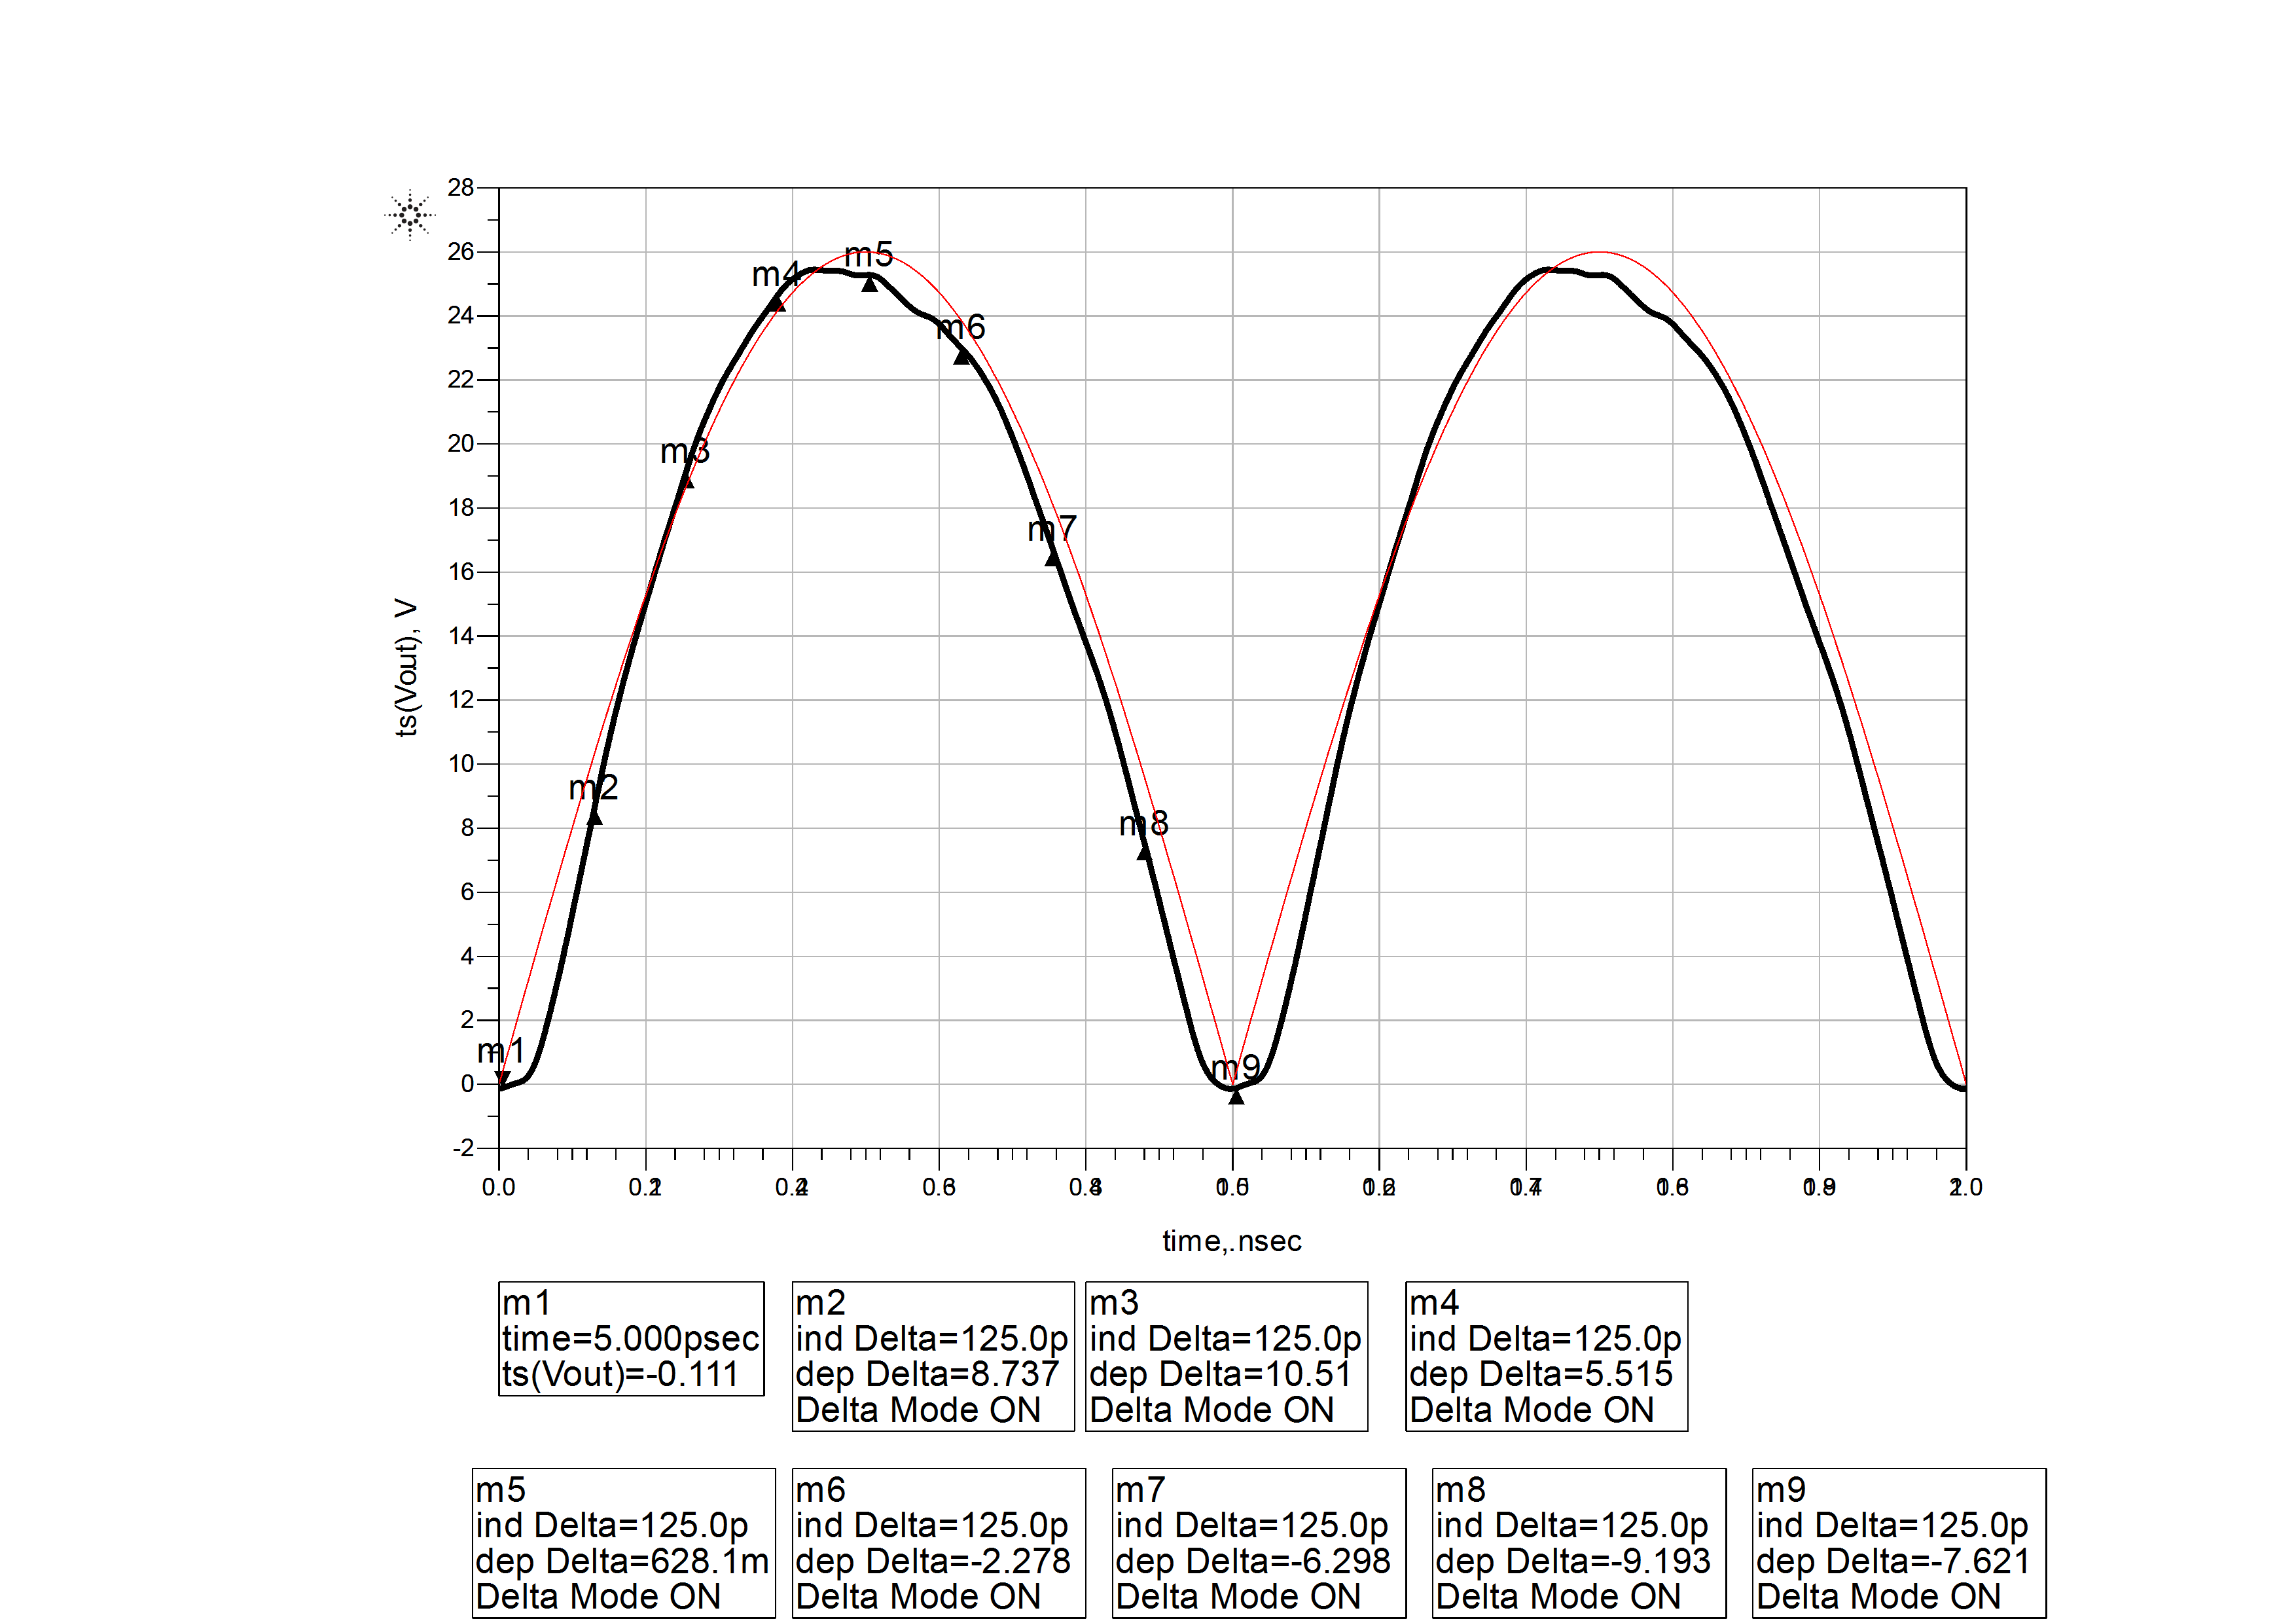
\includegraphics[width=1\textwidth, draft]{halfsine_generated_1GHz.png}
	\caption{Digital to analog converted signal representing a sine half wave and a theoretical signal to compare the signal to noise ratio}
	\label{halfsine}
\end{figure}
